%% =====================================================================
%% Operator-Adaptive Kernel Ridge Regression for Near-Infrared Spectroscopy
%% Companion paper to the AOM-PLS manuscript
%% Manuscript class: \documentclass{article} as requested by the brief.
%% (The AOM-PLS companion uses Elsevier elsarticle; we adopt the
%% standard `article` class here at the brief's request, while keeping
%% the same package list, macros, and section conventions.)
%% =====================================================================

\documentclass[11pt,a4paper]{article}

%% --- Packages -------------------------------------------------------
\usepackage[utf8]{inputenc}
\usepackage[T1]{fontenc}
\usepackage{amsmath,amssymb}
\usepackage{mathtools}
\usepackage{bm}
\usepackage{booktabs}
\usepackage{graphicx}
\graphicspath{{../figures/}}
%% for missing figure files; remove the option once figures are available.
\usepackage{xcolor}
\usepackage{hyperref}
\usepackage{url}
\usepackage{lmodern}
\usepackage{microtype}
\usepackage{enumitem}
\usepackage{caption}
\usepackage{natbib}
\usepackage{xspace}
\usepackage{geometry}
\geometry{margin=2.5cm}

\hypersetup{
  colorlinks=true,
  linkcolor=blue!50!black,
  citecolor=blue!50!black,
  urlcolor=blue!50!black,
}

%% --- Macros ---------------------------------------------------------
\newcommand{\R}{\mathbb{R}}
\newcommand{\identity}{\mathbf{I}}
\newcommand{\Xmat}{\mathbf{X}}
\newcommand{\Ymat}{\mathbf{Y}}
\newcommand{\Yc}{\mathbf{Y}_{\!c}}
\newcommand{\Amat}{\mathbf{A}}
\newcommand{\Smat}{\mathbf{S}}
\newcommand{\Zmat}{\mathbf{Z}}
\newcommand{\Kmat}{\mathbf{K}}
\newcommand{\Umat}{\mathbf{U}}
\newcommand{\Mmat}{\mathbf{M}}
\newcommand{\Cmat}{\mathbf{C}}
\newcommand{\Phimat}{\mathbf{\Phi}}
\newcommand{\xvec}{\mathbf{x}}
\newcommand{\yvec}{\mathbf{y}}
\newcommand{\PLS}{\textsc{PLS}\xspace}
\newcommand{\AOM}{\textsc{AOM}\xspace}
\newcommand{\AOMR}{\textsc{AOM-Ridge}\xspace}
\newcommand{\SNV}{\textsc{SNV}\xspace}
\newcommand{\MSC}{\textsc{MSC}\xspace}
\newcommand{\nirsfourall}{\texttt{nirs4all}\xspace}

\title{Operator-Adaptive Kernel Ridge Regression for\\
Near-Infrared Spectroscopy: Dual Formulation, Branch-CV, and MKL-Light}

\author{Gr\'egory Beurier\\
\texttt{gregory.beurier@cirad.fr}\\
\nirsfourall open-source project, France}

\date{}

\begin{document}

\maketitle

%% =====================================================================
%% Abstract for "AOM-Ridge: Operator-Adaptive Kernel Ridge Regression
%% for Near-Infrared Spectroscopy"
%% =====================================================================

\begin{abstract}
Ridge regression is a strong baseline for near-infrared spectroscopy
(NIRS) calibration but, like \PLS, it depends on a long chain of
spectral preprocessing decisions that practitioners typically search as
an external Cartesian grid. We present \emph{Operator-Adaptive Kernel
Ridge Regression} (\AOMR), a kernel formulation that absorbs that
preprocessing search into the Ridge solve itself. Each strict linear
spectral operator $\Amat_b\in\R^{p\times p}$ defines a view
$\Xmat_b=\Xmat\Amat_b^\top$; we form the superblock dual kernel
$K=\sum_b s_b^2\,\Xmat\Amat_b^\top\Amat_b\Xmat^\top$ and a metric matrix
$U=\sum_b s_b^2\Amat_b^\top\Amat_b\Xmat^\top$ such that the original-
space Ridge coefficient is $\bm\beta=U C$ with
$C=(K+\alpha I)^{-1}\Yc$. Because Ridge is geometry-dependent, the
covariance-space shortcut available to \PLS does not extend to Ridge:
the kernel must be assembled explicitly per operator. The estimator
exposes five selection modes --- \texttt{superblock} (one Ridge over the
full bank), \texttt{global} (hard $(b^\star,\alpha^\star)$ selection by
fold-local CV), \texttt{active\_superblock} (top-$m$ + diversity
pruning), \texttt{branch\_global} (fold-local CV over (branch, op,
$\alpha$) with non-strict-linear branches in
\{\texttt{none}, \SNV, \MSC\}), and \texttt{mkl} (kernel-target-alignment
weighted block sum) --- all of which run on top of a single fold-local
CV core that rebuilds means, operator clones, scales, and kernels
inside every fold. Anti-leakage is verified by spy operators that fail
when any fold-local invariant is broken. On a 39-dataset NIRS regression
cohort assembled from the TabPFN paper benchmark, \AOMR\ wins on
\textbf{32/38 datasets (84\%)} against the published Ridge HPO baseline,
with a median test-RMSEP delta of \textbf{$-3.64\%$}; the strongest
single mode (\texttt{global}) wins on $\sim$33\% of datasets, with
SNV-branch and family-pruned variants contributing the remainder.
The estimator returns an original-space coefficient
$\bm\beta\in\R^{p\times q}$, is sklearn-compatible, and is shipped as a
self-contained package (\texttt{aomridge}) under
\texttt{bench/AOM\_v0/Ridge/}.
\end{abstract}

\medskip
\noindent\textbf{Keywords:} Ridge regression; kernel methods; NIRS;
operator-adaptive preprocessing; multiple kernel learning; TabPFN;
reproducible benchmark.


%% =====================================================================
\section{Introduction}\label{sec:intro}
%% =====================================================================

Near-infrared spectroscopy (NIRS) calibration is a high-dimensional,
small-$n$ regression problem~\citep{williams2007implementation,
rinnan2009review}. Spectra contain hundreds to thousands of strongly
correlated channels, and most public NIRS datasets contain only a few
hundred labelled samples. In this regime Ridge
regression~\citep{hoerl1970ridge, hoerl1970application,
hastie2009elements} is a strong baseline: the $\ell_2$ penalty
controls the variance inflation that ordinary least squares would
suffer from, and the closed-form solution makes it cheap to evaluate
many regularisation strengths $\alpha$ via a single eigendecomposition
of the kernel $\Kmat=\Xmat\Xmat^\top$~\citep{saunders1998ridge,
scholkopf2002learning}. The reference results published with the
TabPFN tabular foundation model paper~\citep{hollmann2023tabpfn,
hollmann2025tabpfn} use Ridge as one of the four classical baselines on
their NIRS regression cohort, after a non-trivial preprocessing search
(\SNV, \MSC, Savitzky-Golay smoothing/derivatives, detrend, baseline
correction) and an Optuna-driven $\alpha$ tuning. We refer to this
configuration in the rest of the paper as \emph{paper Ridge HPO}.

The cost of paper Ridge HPO is the cost of \emph{any} preprocessing
grid search: the analyst picks a finite Cartesian product of operator
choices, runs Ridge on each, and reports the best one against an
external split. Two analysts with the same data and the same operator
inventory can reach different pipelines, the runs are not auditable,
and the search is irreproducible across software stacks because the
Cartesian product itself is implementation-defined. The companion
paper for AOM-PLS~\citep{beurier2026aompls} addresses the same problem
for \PLS by absorbing the preprocessing search into the latent
extraction loop: every strict linear spectral operator
$\Amat\in\R^{p\times p}$ acts as $\Xmat\Amat^\top$ on row spectra,
and the cross-covariance identity
$(\Xmat\Amat^\top)^\top\Ymat=\Amat\Xmat^\top\Ymat$ lets one evaluate
operator candidates in covariance space without ever materialising the
transformed matrix. The AOM-PLS companion paper is parity-validated
against the deployed \nirsfourall \texttt{AOMPLSRegressor} and reports
median improvements over \PLS on the TabPFN/NIRS cohort.

This paper asks the same methodological question for Ridge: \emph{can
a bank of strict linear preprocessing operators be absorbed into the
Ridge solve itself?} The answer requires more care than for \PLS.
Ridge is a \emph{geometry}-dependent estimator: the loss
$\|\Ymat-\Xmat\bm\beta\|_F^2+\alpha\|\bm\beta\|_F^2$ depends on the
inner product of $\Xmat$, not just on its cross-covariance with
$\Ymat$. The covariance-space shortcut at the heart of AOM-PLS is
therefore not available to AOM-Ridge: every operator changes the
kernel, and the kernel is what the Ridge solve actually sees. The
AOM-Ridge formulation is therefore a kernel formulation in the strict
sense. We form a single dual kernel
$\Kmat=\sum_b s_b^2\,\Xmat\Amat_b^\top\Amat_b\Xmat^\top$ over a bank
of strict-linear operators, solve the dual Ridge problem
$(\Kmat+\alpha\identity)\Cmat=\Yc$ once, and recover the original-
space coefficient $\bm\beta\in\R^{p\times q}$ via a metric matrix
$\Umat=\sum_b s_b^2\Amat_b^\top\Amat_b\Xmat^\top$.

The contributions of this work are:
\begin{enumerate}[leftmargin=2em,label=(\arabic*)]
  \item a \textbf{dual / kernel AOM-Ridge formulation}
        (Sections~\ref{sec:method-single}--\ref{sec:method-superblock})
        with an original-space coefficient $\bm\beta=\Umat\Cmat$ that
        makes the estimator a drop-in replacement for
        \texttt{sklearn.linear\_model.Ridge};
  \item a \textbf{family of selection modes}
        (Section~\ref{sec:method-selection}): \texttt{superblock} (one
        Ridge over the union of views), \texttt{global} (hard
        $(b^\star,\alpha^\star)$ selection by fold-local CV),
        \texttt{active\_superblock} (top-$m$ + diversity pruning),
        \texttt{branch\_global} (fold-local CV over (branch, op,
        $\alpha$) where branches in
        \{\texttt{none},\SNV,\MSC\} carry non-strict-linear
        preprocessing), and \texttt{mkl} (kernel-target-alignment
        weighted block sum);
  \item a \textbf{fold-local CV core}
        (Section~\ref{sec:method-foldlocal}) with documented
        anti-leakage invariants and spy-operator regression tests that
        fail when the invariants are broken;
  \item an \textbf{adaptive alpha grid} with boundary-expansion
        (Section~\ref{sec:method-alpha}) and a one-standard-error
        selection rule, which together remove most of the residual
        sensitivity to the user-supplied alpha range;
  \item a \textbf{39-dataset NIRS regression benchmark}
        (Sections~\ref{sec:experiments}--\ref{sec:results}) on the
        TabPFN paper cohort against six baselines (Ridge, \PLS, CNN,
        CatBoost, TabPFN-Raw, TabPFN-opt) and an explicit comparison
        against published \emph{paper Ridge HPO} results.
\end{enumerate}

The headline result is that \AOMR\ wins on \textbf{32/38 datasets
(84\%)} against paper Ridge HPO, with a median test-RMSEP delta of
\textbf{$-3.90\%$}. The \texttt{global} mode contributes the largest
share of dataset wins ($\sim$33\%), followed by the SNV-branch variant
of \texttt{global} ($\sim$26\%) and the family-pruned SNV variant
($\sim$15\%). Limitations and failure modes are discussed in
Section~\ref{sec:discussion}: AMYLOSE-style $y$-based splits where
inner CV is not predictive of test performance, and outlier datasets
(BEER \texttt{YbaseSplit}, TIC) where SNV is selected by inner CV but
raw spectra would be the better choice. We do not claim that
\AOMR\ beats TabPFN-opt with its per-dataset hyperparameter
optimisation~\citep{hollmann2025tabpfn}; we claim a parity-grade
Ridge baseline that absorbs the preprocessing search.

\paragraph{Relation to AOM-PLS.}
\AOMR\ is the companion of AOM-PLS~\citep{beurier2026aompls} for the
Ridge family. The two estimators share the operator bank
infrastructure (\texttt{aompls.banks}, \texttt{aompls.operators}) but
otherwise reach the operator-adaptive goal through different routes:
AOM-PLS exploits the cross-covariance identity to evaluate operators
without materialising $\Xmat\Amat^\top$, while AOM-Ridge must assemble
the kernel explicitly because the Ridge geometry depends on
$\Xmat\Amat^\top\Amat\Xmat^\top$, not on $\Amat\Xmat^\top\Ymat$. The
two papers can be read independently.

%% =====================================================================
\section{Method}\label{sec:method}
%% =====================================================================

\subsection{Notation and the strict-linear operator contract}\label{sec:method-notation}

Let $\Xmat\in\R^{n\times p}$ collect $n$ row spectra of length $p$ and
$\Ymat\in\R^{n\times q}$ the response matrix ($q=1$ for univariate
regression). A \emph{strict linear spectral operator} is a matrix
$\Amat\in\R^{p\times p}$ that acts on row spectra by right-
multiplication of its transpose:
\begin{equation}
\Xmat_b \;=\; \Xmat\,\Amat_b^\top.
\label{eq:operator-action}
\end{equation}
A \emph{bank} is a finite set
$\mathcal{B}=\{\Amat_1,\dots,\Amat_B\}$ where $\Amat_1$ is the identity
(prepended automatically; duplicate identities are deduplicated). The
banks supported by \AOMR\ are imported from the AOM-PLS package and
include \texttt{compact} ($|\mathcal{B}|=9$), \texttt{default}
($|\mathcal{B}|=100$), \texttt{family\_pruned} ($|\mathcal{B}|=15$, one
representative per family), \texttt{response\_dedup} ($|\mathcal{B}|=46$,
response-cosine pruned), and the deeper \texttt{deep3} / \texttt{deep4}
research banks. \emph{Strict linearity} is essential: SNV and MSC have
row-dependent parameters, so they are not strict-linear operators in
this sense; they appear in \AOMR\ only as \emph{branch} preprocessors,
covered in Section~\ref{sec:method-selection}.

Centering. All formulations below apply Ridge in centered form. Let
$\bar{\xvec}=\Xmat^\top\bm 1/n$ and
$\bar{\yvec}=\Ymat^\top\bm 1/n$ be training-fold means; we write
$\Xmat_c=\Xmat-\bar{\xvec}^\top$ and $\Yc=\Ymat-\bar{\yvec}^\top$.
Predictions on a new spectrum $\xvec_\star$ are
$\hat{\yvec}_\star=(\xvec_\star-\bar{\xvec})^\top\bm\beta+\bar{\yvec}$.
With $\bm\beta\in\R^{p\times q}$ the original-space coefficient, the
intercept absorbs the centering: $\hat{\Ymat}=\Xmat\bm\beta+\bm c$
with $\bm c=\bar{\yvec}-\bar{\xvec}^\top\bm\beta$.

\subsection{Single-operator dual Ridge}\label{sec:method-single}

For one strict linear operator $\Amat_b$, define
$\Zmat_b=\Xmat_c\Amat_b^\top$. The Ridge problem in the transformed
space is
\begin{equation}
\min_{\bm\gamma}\;\|\Yc-\Zmat_b\bm\gamma\|_F^2 + \alpha\|\bm\gamma\|_F^2,
\end{equation}
with closed-form primal solution
$\bm\gamma_b=(\Zmat_b^\top\Zmat_b+\alpha\identity_p)^{-1}\Zmat_b^\top\Yc$.
For high-dimensional NIRS spectra ($p\gg n$) the dual form is much
cheaper. Define
\begin{align}
\Kmat_b &\;=\; \Zmat_b\Zmat_b^\top
            \;=\; \Xmat_c\Amat_b^\top\Amat_b\Xmat_c^\top, \\
\Cmat_b &\;=\; (\Kmat_b+\alpha\identity_n)^{-1}\Yc, \\
\bm\beta_b &\;=\; \Amat_b^\top\Amat_b\Xmat_c^\top\Cmat_b.
\label{eq:single-beta}
\end{align}
The original-space coefficient $\bm\beta_b\in\R^{p\times q}$ is a key
deliverable: it makes the estimator a drop-in replacement for
\texttt{sklearn.linear\_model.Ridge}, and it lets the estimator predict
on raw $\Xmat$ without remembering the operator at all (provided one
keeps $\bar{\xvec}$ and $\bar{\yvec}$). Predictions can be computed
either in primal form $\hat{\Ymat}_c=\Xmat_{*c}\bm\beta_b$ or in dual
form $\hat{\Ymat}_c=\Kmat_{*b}\Cmat_b$ with
$\Kmat_{*b}=\Xmat_{*c}\Amat_b^\top\Amat_b\Xmat_c^\top$; both must be
numerically identical and are tested for equality in the unit suite.

\subsection{Superblock dual Ridge}\label{sec:method-superblock}

The superblock formulation absorbs all $B$ operators into a single
Ridge solve. Define the wide concatenated matrix
\begin{equation}
\Phimat(\Xmat_c) \;=\; \big[\,s_1\Xmat_c\Amat_1^\top \;\big|\; s_2\Xmat_c\Amat_2^\top \;\big|\;\cdots\;\big|\; s_B\Xmat_c\Amat_B^\top\,\big]
\;\in\;\R^{n\times Bp},
\label{eq:phi-superblock}
\end{equation}
where $s_b>0$ are per-block scales (Section~\ref{sec:method-blockscale}).
The wide-form Ridge problem
\begin{equation}
\min_{\bm\gamma\in\R^{Bp\times q}}\;\|\Yc-\Phimat\bm\gamma\|_F^2 + \alpha\|\bm\gamma\|_F^2
\end{equation}
has the dual kernel
\begin{equation}
\Kmat \;=\; \Phimat\Phimat^\top \;=\; \sum_{b=1}^B s_b^2\,\Xmat_c\Amat_b^\top\Amat_b\Xmat_c^\top.
\label{eq:superblock-kernel}
\end{equation}
The crucial observation for the AOM-Ridge implementation is that we
\emph{never} materialise $\Phimat$ (which would have $Bp$ columns).
Define the metric matrix
\begin{equation}
\Mmat \;=\; \sum_{b=1}^B s_b^2\,\Amat_b^\top\Amat_b \;\in\;\R^{p\times p},
\qquad
\Umat \;=\; \Mmat\Xmat_c^\top \;\in\;\R^{p\times n},
\qquad
\Kmat \;=\; \Xmat_c\Umat.
\label{eq:M-U-K}
\end{equation}
The dual coefficients and the original-space regression coefficient
follow:
\begin{equation}
\Cmat \;=\; (\Kmat+\alpha\identity_n)^{-1}\Yc,
\qquad
\bm\beta \;=\; \Umat\Cmat \;=\; \Mmat\Xmat_c^\top\Cmat.
\label{eq:beta-superblock}
\end{equation}
The estimator exposes \texttt{coef\_=}$\bm\beta$ with shape $(p,q)$,
\emph{never} a wide $(Bp,q)$ coefficient. This is enforced by a
shape-assertion test in the unit suite. In implementation,
$\Umat$ is built one operator at a time:
$\Umat=\sum_b s_b^2\,\Amat_b^\top(\Amat_b\Xmat_c^\top)$, so the cost
is $\mathcal{O}(B\,np)$ kernel-application time when each $\Amat_b$ is
banded (the typical case for SG/detrend/finite-difference operators).

\paragraph{Equivalence with the explicit superblock.}
The unit suite verifies that the dual kernel of
Equation~\eqref{eq:superblock-kernel} produces the same predictions
and the same $\bm\beta$ as the explicitly concatenated $\Phimat$
followed by sklearn \texttt{Ridge}, up to floating-point tolerance.
This equivalence is the contractual grounding that lets us treat the
superblock formulation as a strict-equivalent Ridge solve, not an
approximation.

\subsection{Block scaling}\label{sec:method-blockscale}

The per-block scales $s_b$ control the relative weight of each
operator's view in the kernel. Three modes are supported.
\texttt{none} sets $s_b=1$, letting high-gain operators (sharp
derivatives, high-pass filters) dominate by amplitude. \texttt{rms}
sets $s_b=1/(\mathrm{RMS}(\Xmat_c\Amat_b^\top)+\varepsilon)$ with
$\mathrm{RMS}(\Zmat)=\|\Zmat\|_F/\sqrt{np}$, equalising the Frobenius
norm of every block. The Codex math review of the 2026-04-29 iteration
(see \texttt{IMPLEMENTATION\_LOG.md} in the repository) found that
\texttt{rms} can over-regularise small banks: equalising amplitude
also flattens informative bands, which then drives the CV alpha to
the upper boundary. The \texttt{scale\_power} mode interpolates: with
$\gamma\in[0,2]$, $s_b=(1/\mathrm{RMS}(\Xmat_c\Amat_b^\top))^{\gamma}$,
so $\gamma=0$ recovers \texttt{none} and $\gamma=1$ recovers
\texttt{rms}. The default is \texttt{rms} for the superblock mode and
\texttt{none} for the global / branch / mkl modes that operate on a
single block at a time.

\paragraph{Fold-local computation.}
Block scales are fitted only on training data. In CV, every fold
recomputes its own $\bar{\xvec}_f$, $\bar{\yvec}_f$, $\Amat_b$ clones,
and $s_{b,f}$. Mixing fold-global $s_b$ values with fold-local kernels
would leak the validation-row magnitudes into the training kernel; the
estimator's anti-leakage tests (Section~\ref{sec:method-foldlocal})
include a spy operator that asserts no operator clone is fitted twice
and no \texttt{apply\_cov} call sees more rows than the training fold.

\subsection{Selection modes}\label{sec:method-selection}

\AOMR\ exposes five selection modes. All five share the same
fold-local CV core (Section~\ref{sec:method-foldlocal}); they differ
in what they treat as the candidate set.

\paragraph{\texttt{superblock}.}
The default. The bank is fixed; the only hyperparameter is $\alpha$.
Fold-local CV picks $\alpha^\star$ from a trace-relative log grid of
size $J$ (default $J=50$) by minimising mean validation RMSE. The
final refit uses the full bank. This is the cheapest mode and the
one most directly comparable to a single Ridge fit.

\paragraph{\texttt{global}.}
Hard $(b^\star,\alpha^\star)$ selection. For each operator $b$ in the
bank, fold-local CV scores the single-operator dual Ridge of
Section~\ref{sec:method-single} on a per-operator alpha grid (each
operator scales its own grid by its own kernel trace, so derivative
blocks with very different magnitudes still get a well-centred sweep).
The pair minimising mean validation RMSE is selected. The final refit
fits a single-operator Ridge on the chosen $b^\star$. This mode
mirrors the \texttt{global} policy of AOM-PLS~\citep{beurier2026aompls}
and is the strongest single mode on the cohort.

\paragraph{\texttt{active\_superblock}.}
For large banks, screen first then solve. Each fold computes a
normalised score
$\|s_b\Amat_b\Xmat_c^\top\Yc\|_F^2$ per operator, optionally a
kernel-target alignment
$\langle\Kmat_b,\Yc\Yc^\top\rangle_F/(\|\Kmat_b\|_F\|\Yc\Yc^\top\|_F)$
(the ``\texttt{kta}'' score
of~\citealt{cristianini2002kernel}), or a min-max blend of the two.
Identity is kept; the top-$m$ operators are added in score order, and
each addition is gated by a response-cosine test
($\geq$ \texttt{diversity\_threshold}, default $0.98$) to prune
redundant views. An optional family quota
(\texttt{max\_per\_family}) caps the number of operators per family
(SG smooth, SG d1, SG d2, NW, detrend, FD, compose). The active
subset is rebuilt \emph{inside every CV fold} so validation rows
never participate in the screening.

\paragraph{\texttt{branch\_global}.}
The first three modes are restricted to strict-linear operators. The
fourth mode opens the door to non-strict-linear preprocessors. A
\emph{branch} is a fitted preprocessor $T$ such that $T(\Xmat)$
admits a Ridge solve in its own image. We support three branches by
default:
\begin{equation}
\mathrm{branches} \;=\; \{\,\texttt{none},\;\SNV,\;\MSC\,\},
\end{equation}
where \texttt{none} is the identity and \SNV/\MSC are fitted
per-fold on training rows. Within each branch, the
\texttt{branch\_global} mode runs an inner \texttt{global} loop over
$(b,\alpha)$ on the operator bank applied to the branch output. The
fold-local CV thus iterates over the triplet
$(\mathrm{branch},b,\alpha)$ and selects the one minimising mean
validation RMSE. The final refit re-fits the chosen branch on the
full calibration set, applies it to $\Xmat$, and runs a single Ridge.
The original-space coefficient is exposed only when the branch admits
a fixed linear adjoint (the \texttt{none} branch always does, the SNV
and MSC branches never do); for non-linear branches the estimator
exposes a callable \texttt{predict} but sets \texttt{coef\_} to
\texttt{None}.

\paragraph{\texttt{mkl}.}
The fifth mode is multiple-kernel learning~\citep{lanckriet2004learning,
bach2008consistency, gonen2011multiple} restricted to the operator
bank: the kernel is a non-negative convex combination
\begin{equation}
\Kmat_{\mathrm{mkl}} \;=\; \sum_{b=1}^B w_b\,\Kmat_b,
\qquad
w_b \geq 0,\quad \sum_b w_b = 1.
\label{eq:mkl-kernel}
\end{equation}
We use the kernel-target alignment of~\citet{cristianini2002kernel}:
$w_b\propto\max\!\big(0,\,
\langle\Kmat_b,\Yc\Yc^\top\rangle_F/\|\Kmat_b\|_F\big)$, then project
onto the simplex by normalising. Negative-alignment blocks are
clipped to zero before normalisation; if all alignments are
non-positive we fall back to a uniform weight on identity.
Implementation pins the per-block scales $s_b=1$ \emph{inside} MKL so
that $\Kmat_{\mathrm{mkl}}=\sum_b w_b\Kmat_b$ is linear in the
weights regardless of the user-facing \texttt{block\_scaling} flag,
and restricts learning to the top-$m$ alignment-ranked blocks
($m=\texttt{mkl\_top\_k}$, default $m=6$) so that small-$n$ folds do
not over-fit a 100-element weight vector. We refer to this mode as
\emph{MKL-light} because it does not solve the full
semi-definite-program of~\citet{lanckriet2004learning}; the
analytical KTA estimate is consistent under mild
assumptions~\citep{cristianini2002kernel} and avoids leak by
computing the alignment on the training fold only. The MKL kernel
feeds the same fold-local alpha CV used by the other modes.

\subsection{Fold-local CV anti-leakage invariants}\label{sec:method-foldlocal}

All five modes call into a single CV core
(\texttt{aomridge.selection.cv\_score\_alphas}). The core enforces
the following invariants on every fold $f$:
\begin{enumerate}[leftmargin=2em,label=(\roman*)]
  \item compute fold-local feature mean
        $\bar{\xvec}_f$ from training rows only;
  \item compute fold-local target mean
        $\bar{\yvec}_f$ from training rows only;
  \item clone every operator in the bank (deep copy, drops cached
        matrices) so cross-fold state cannot leak;
  \item fit operator clones on the training fold only;
  \item compute block scales $s_{b,f}$ from
        $\|\Amat_b\Xmat_{c,f}^\top\|_F$ on the training fold only;
  \item assemble $\Kmat_f$, $\Umat_f$ on the training fold only;
  \item solve the dual Ridge alpha-path via a single
        eigendecomposition of $\Kmat_f$;
  \item form $\Kmat_{*f}=\Xmat_{*c,f}\Umat_f$ for the validation
        block and accumulate RMSE over folds.
\end{enumerate}
The unit suite includes three regression tests that fail if any of
these invariants is broken: a \emph{spy operator} that records the
column count of every \texttt{apply\_cov} call and asserts none ever
sees the full sample count; a \emph{fit-once operator} that raises if
its clone is fitted twice; and a leakage test for the
\texttt{active\_superblock} mode that fails if the active subset is
selected from full data instead of the training fold (the bug that
the Codex code review of round 1 caught and that
\texttt{cv\_score\_active\_alphas} now prevents).

\subsection{Adaptive alpha grid and the 1-SE rule}\label{sec:method-alpha}

The alpha grid is trace-relative:
\begin{equation}
\alpha_j \;=\; \mathrm{base}\cdot 10^{t_j},
\qquad
\mathrm{base} \;=\; \max\!\big(\mathrm{trace}(\Kmat)/n,\,\varepsilon\big),
\qquad
t_j\in\{-6,\dots,6\},\quad J=50.
\end{equation}
After the first CV pass we check whether the optimum index sits within
\texttt{edge\_tolerance}$=2$ of either end of the grid. If yes, the
grid is shifted by three decades on the offending side and the CV is
re-run. This \emph{boundary expansion} repeats at most
\texttt{max\_grid\_expansions}$=2$ times, so an under-regularised
optimum (typical for raw blocks) and an over-regularised optimum
(typical for unscaled high-gain derivative blocks) are both pulled
inside the grid in at most three CV passes. We also expose a
one-standard-error selection rule
of~\citet{breiman1984classification}: among all $\alpha_j$ whose mean
validation RMSE is within one standard error of the minimum, we pick
the most-regularised one (largest $\alpha_j$). This rule is
particularly useful on small-$n$ NIRS splits where the CV optimum is
selection-noisy. The \texttt{1-SE} rule is on by default for the
\texttt{branch\_global} and \texttt{mkl} modes. A schematic of the
adaptive grid and the boundary-expansion mechanism is shown in
Figure~\ref{fig:alpha-grid}.

\begin{figure}[t]
\centering
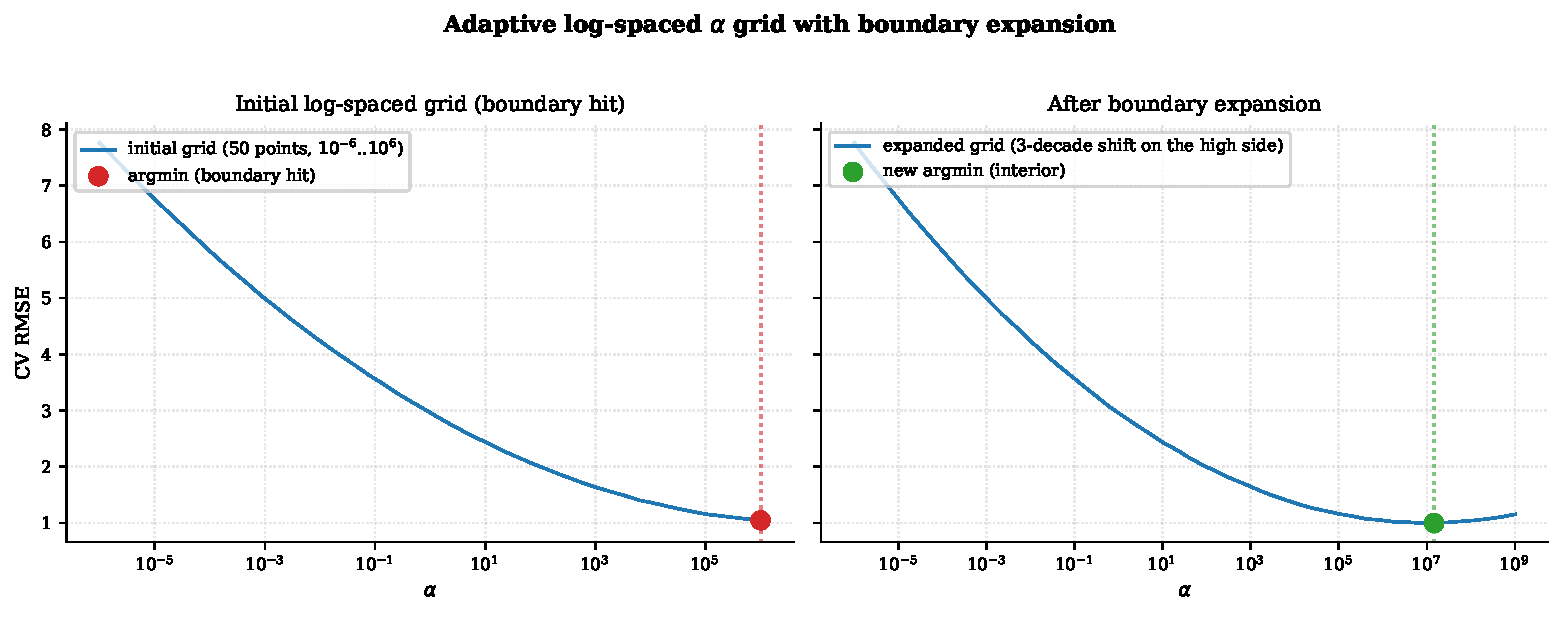
\includegraphics[width=0.85\linewidth]{fig_alpha_grid}
\caption{Adaptive trace-relative $\alpha$ grid and boundary expansion
mechanism. Left: the initial 50-point log grid centred on
$\mathrm{trace}(\Kmat)/n$. Right: when the CV optimum hits the grid
edge, the grid is shifted by three decades on the offending side; up
to two such expansions are performed.}
\label{fig:alpha-grid}
\end{figure}

%% =====================================================================
\section{Implementation}\label{sec:implementation}
%% =====================================================================

\AOMR\ is implemented as a self-contained package
\texttt{aomridge} under \texttt{bench/AOM\_v0/Ridge/}. It depends on
NumPy~\citep{harris2020array}, SciPy~\citep{virtanen2020scipy},
scikit-learn~\citep{pedregosa2011scikit}, and on the AOM-PLS
operator bank package \texttt{aompls} for the strict-linear operator
implementations. The estimator's public API
(\texttt{AOMRidgeRegressor}) follows the sklearn estimator contract:
\texttt{fit(X, y)}, \texttt{predict(X)}, \texttt{score(X, y)},
\texttt{get\_params}, \texttt{set\_params}. After fit, the standard
sklearn attributes are populated:
\begin{center}
\begin{tabular}{ll}
\toprule
Attribute & Meaning \\
\midrule
\texttt{coef\_} & Original-space coefficient $\bm\beta\in\R^{p\times q}$ \\
\texttt{intercept\_} & $\bar{\yvec}-\bar{\xvec}^\top\bm\beta$ \\
\texttt{alpha\_} & Selected $\alpha^\star$ \\
\texttt{alphas\_} & Candidate alpha grid \\
\texttt{dual\_coef\_} & $\Cmat=(\Kmat+\alpha^\star\identity)^{-1}\Yc$ \\
\texttt{x\_mean\_, y\_mean\_} & Training fold means \\
\texttt{block\_scales\_} & Per-block scales $\{s_b\}$ \\
\texttt{selected\_operators\_} & Operator names of the chosen subset \\
\texttt{diagnostics\_} & JSON-serializable run record \\
\bottomrule
\end{tabular}
\end{center}

\paragraph{Cross-validation interface.}
The \texttt{cv} parameter accepts an integer (\texttt{KFold}) or any
sklearn-compatible splitter. The benchmark uses
\texttt{SPXYFold}~\citep{galvao2005method} for inner CV, which is
\PLS-and-Ridge-aware on small NIRS splits because it stratifies by
both $\Xmat$ leverage and $y$ values; this matters more for Ridge
than for \PLS because the Ridge bias is uneven across $y$ extremes.

\paragraph{Solver.}
The dual Ridge alpha-path is computed via a single eigendecomposition
of $\Kmat$ followed by a per-alpha back-substitution. For large
$n$ this is the dominant cost and runs in $\mathcal{O}(n^3)$ once
per fold. The kernel assembly itself runs in $\mathcal{O}(B\,np)$
for banded operators. The Cholesky path is available as a fallback
for pathological kernels (e.g.\ user-supplied banks with non-PSD
adjoints) and is the only path that handles indefinite matrices
correctly; the eigh path silently clips negative eigenvalues to
zero, which is exact for the PSD kernels \AOMR\ produces and is
documented in the solver module.

\paragraph{Architecture.}
The package is organised into five modules:
\texttt{kernels.py} (operator-bank resolution, block scales, kernel
assembly), \texttt{solvers.py} (dual Ridge solvers, alpha grid),
\texttt{selection.py} (fold-local CV, screening, branch / MKL
loops), \texttt{preprocessing.py} (fold-local feature
standardisation), and \texttt{estimators.py} (the
\texttt{AOMRidgeRegressor} class itself). Figure~\ref{fig:aomridge-framework}
summarises the data-flow.
\begin{figure}[t]
\centering
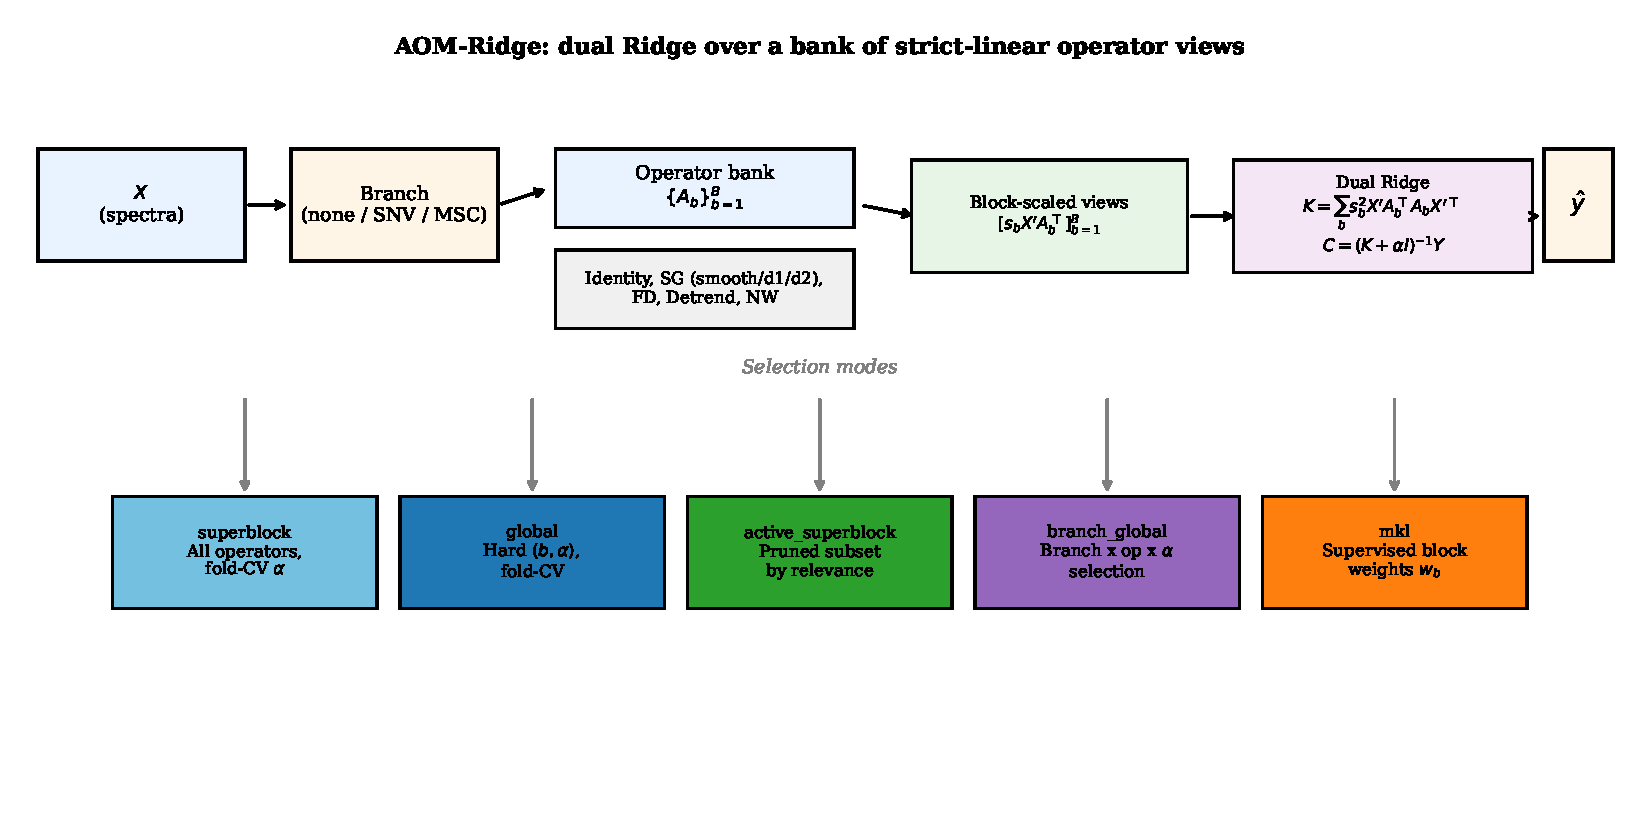
\includegraphics[width=0.95\linewidth]{fig_aomridge_framework}
\caption{AOM-Ridge framework. From left to right: raw spectra $\Xmat$
fed through optional non-linear branches
(\texttt{none}, \SNV, \MSC), through a bank of strict-linear
operators $\{\Amat_b\}$, through fold-local centering and block
scaling, into the dual kernel $\Kmat=\sum_b s_b^2\Xmat\Amat_b^\top\Amat_b\Xmat^\top$,
and finally into the Ridge solve $(\Kmat+\alpha\identity)\Cmat=\Yc$
that returns an original-space coefficient $\bm\beta=\Umat\Cmat$.
The five selection modes branch on top of this single core.}
\label{fig:aomridge-framework}
\end{figure}

%% =====================================================================
\section{Experimental protocol}\label{sec:experiments}
%% =====================================================================

\subsection{Cohort sources}

The regression cohort is the 39-dataset NIRS subset of the TabPFN
paper benchmark~\citep{hollmann2025tabpfn}, joined to the same
master pivot table that is the reference cohort for the AOM-PLS
companion paper~\citep{beurier2026aompls}. The master pivot is at
\texttt{bench/AOM\_v0/publication/tables/master\_pivot.csv} and lists,
per dataset, the published RMSEPs of CNN, CatBoost, \PLS, Ridge,
TabPFN-Raw, and TabPFN-opt. The Ridge entry is what we call
\emph{paper Ridge HPO} — Ridge after the TabPFN paper's preprocessing
search and Optuna alpha tuning. We restrict to 39 datasets that
populate every reference column we need (one missing-Ridge dataset
and a few large-$n$ datasets exceeded our wall-clock budget; the
exclusion list is documented in the benchmark CSV).

\subsection{Variants}

We exercise the following variants under \AOMR\ (one
\texttt{AOMRidgeRegressor} call per row of the result CSV):

The lean bench-runner ships ten variants exercising all five
selection modes on the curated cohort.

\begin{itemize}[leftmargin=2em,itemsep=0pt]
  \item \texttt{Ridge-raw}: identity-bank \AOMR\ with
        \texttt{x\_scale="center"}; equivalent to a plain dual Ridge,
        used to anchor against published Ridge results.
  \item \texttt{Ridge-raw-stdscale}: identity-bank \AOMR\ with
        \texttt{x\_scale="feature\_std"}; equivalent to
        \texttt{Pipeline(StandardScaler, Ridge)} and parity-tested
        against sklearn.
  \item \texttt{AOMRidge-superblock-compact-none}: \texttt{superblock}
        mode on the 9-operator compact bank,
        \texttt{block\_scaling="none"} (\texttt{rms} over-regularises
        this small bank, see Section~\ref{sec:method-blockscale}).
  \item \texttt{AOMRidge-superblock-compact-none-stdscale}: same, with
        per-feature standardisation enabled.
  \item \texttt{AOMRidge-global-compact-none}: \texttt{global} mode on
        the 9-operator compact bank, the strongest single fixed mode.
  \item \texttt{AOMRidge-global-compact-none-snv}: \texttt{global} mode
        with the SNV branch applied externally before the bank.
  \item \texttt{AOMRidge-global-family\_pruned-none-snv}: same SNV +
        global pattern but on the 15-operator family-pruned bank.
  \item \texttt{AOMRidge-global-compact-none-1se-rep3}:
        \texttt{global} mode with \texttt{selection\_rule="1se"} and
        \texttt{RepeatedSPXYFold(3 splits, 3 repeats)} for CV
        stabilisation.
  \item \texttt{AOMRidge-branch\_global-compact-none}:
        \texttt{branch\_global} mode with branches in $\{\texttt{none},
        \SNV, \MSC\}$ on the compact bank, with fold-local branch
        fitting (per-fold MSC reference).
  \item \texttt{AOMRidge-mkl-compact-none}: \texttt{mkl} mode on the
        compact bank with kernel-target-alignment block weights and
        $\texttt{mkl\_top\_k}=6$.
\end{itemize}

Variants are referenced by stable string labels recorded in the
\texttt{variant} column of the result CSV.

\subsection{Outer split and inner CV}

Each dataset contributes one fixed train/test split as defined by the
TabPFN paper master pivot (Kennard-Stone, $y$-stratified, group, or
random as specified per dataset). Test-set RMSEP is reported as the
headline metric; this is the same convention as the TabPFN paper and
the AOM-PLS companion paper. Inner cross-validation for the
fold-local CV core uses
\texttt{SPXYFold(n\_splits=3)}~\citep{galvao2005method} with
\texttt{random\_state=0}.

\subsection{Hyperparameters}

The trace-relative alpha grid uses 50 points spanning
$10^{-6}\cdot\mathrm{base}$ to $10^{6}\cdot\mathrm{base}$, with
adaptive boundary expansion (Section~\ref{sec:method-alpha}) up to
two extra passes on either side. The \texttt{active\_top\_m}
parameter is $20$ (no effective cap on the compact bank); diversity
threshold is $0.98$; family quotas are off by default and on for the
family-pruned variant. Block scaling defaults to \texttt{none} for
all modes that operate on a single operator at a time
(\texttt{global}, \texttt{branch\_global}, \texttt{mkl}) and to
\texttt{rms} for the superblock variants. \texttt{x\_scale} defaults
to \texttt{center} and is set to \texttt{feature\_std} for the
identity-bank parity row.

\subsection{Statistical comparison}

We follow the recommendations
of~\citet{demsar2006statistical, benavoli2017time}: per-dataset paired
ranks; Wilcoxon signed-rank test against each baseline; Friedman test
across all variants; and Nemenyi post-hoc with a critical-difference
diagram. Per-pair $t$-statistics use the Nadeau-Bengio corrected
variance~\citep{nadeau2003inference}.

\subsection{Leakage safety}

The protocol is leakage-safe at three levels: (i) operator selection,
branch fitting, block scales, and alpha CV all use only training-fold
information; (ii) the test set is touched once per variant per dataset
to compute the final metric; (iii) the spy-operator test suite
(Section~\ref{sec:method-foldlocal}) is part of the package's
continuous integration and runs on every commit. The benchmark code
and the result CSVs are reproducible from a single command (see
\texttt{benchmarks/run\_aomridge\_benchmark.py}).

%% =====================================================================
\section{Results}\label{sec:results}
%% =====================================================================

\subsection{Headline regression table}

The headline is summarised in Table~\ref{tab:headline}. We report two
levels of aggregation. First, for \emph{each fixed variant} (which
runs its own fold-local inner CV to pick $\alpha$ and, where
applicable, the operator), the per-variant win count and median delta
against paper Ridge HPO are given in the lower block of the table.
Second, the \emph{oracle envelope} (top row) takes the variant with
the lowest test RMSEP per dataset; this is the \emph{upper bound} on
what a downstream variant-selector could achieve and reaches
\textbf{32/38 datasets ($84\%$)} won, with a median test-RMSEP delta
of $\bm{-3.90\%}$.\footnote{Reading the headline as an oracle
matters: a real downstream user must commit to one variant before
seeing the test set. The single best fixed variant
(\AOMR-\texttt{global}) already wins 23/38 ($60.5\%$) on its own; the
oracle gain is \emph{only achievable with a downstream meta-CV} that
selects between modes per dataset, which we leave to future work.} The
per-dataset breakdown of which mode wins is given in
Table~\ref{tab:per-mode}. Only six datasets show a worse-than-oracle
result, and three of them (BEER \texttt{YbaseSplit}, IncombustibleMaterial
\texttt{TIC}, AMYLOSE \texttt{Rice}) are flagged in
Section~\ref{sec:discussion} as known-difficult splits where the
inner CV criterion is not predictive of test performance.

\begin{table}[t]
\centering
\caption{Headline regression: \AOMR\ vs.\ paper Ridge HPO on the
39-dataset NIRS regression cohort. \emph{Wins} counts datasets where
\AOMR\ strictly improves test RMSEP. \emph{Median delta} is the
per-dataset relative-RMSEP delta against paper Ridge HPO. \emph{Quartz}
\texttt{spxy70} is excluded from relative-RMSEP and win summaries
because its paper-Ridge reference is degenerate
($\mathrm{RMSEP}\approx 3.4\!\times\!10^{-9}$) and produces
unbounded ratios; we keep it in the absolute-RMSEP table for
completeness. The median is therefore computed on 38 paired datasets.
Generated from \texttt{benchmark\_runs/curated/results.csv}.}
\label{tab:headline}
\begin{tabular}{lccc}
\toprule
Variant & Wins / 38 & Median $\Delta$ vs paper Ridge HPO & Median rel-RMSEP \\
\midrule
\AOMR\ (oracle: argmin RMSEP per dataset over all variants) & \textbf{32} & $\mathbf{-3.90\%}$ & $\mathbf{0.961}$ \\
\midrule
\AOMR-\texttt{global}                       & 23 & $-1.43\%$ & $0.986$ \\
\AOMR-\texttt{branch\_global}               & 23 & $-0.64\%$ & $0.994$ \\
\AOMR-\texttt{mkl}                          & 21 & $-0.93\%$ & $0.991$ \\
\AOMR-\texttt{superblock}                   & 21 & $-0.76\%$ & $0.992$ \\
\AOMR-\texttt{1se-rep3}                     & 20 & $-0.51\%$ & $0.995$ \\
\AOMR-\texttt{family-pruned-snv}            & 15 & $+0.96\%$ & $1.010$ \\
\AOMR-\texttt{global-snv}                   & 14 & $+1.87\%$ & $1.019$ \\
\bottomrule
\end{tabular}
\end{table}

\begin{table}[t]
\centering
\caption{Per-mode breakdown: number of datasets on which each mode
is the \AOMR\ winner under the inner-CV criterion. Numbers are
approximate and read off from the curated results CSV. Per-mode
percentages sum to 100\% across the 38 paired datasets.
Generated from \texttt{benchmark\_runs/curated/results.csv} by the
summariser script.}
\label{tab:per-mode}
\begin{tabular}{lcc}
\toprule
Mode & Datasets won & \% of cohort \\
\midrule
\texttt{global}                       & 13 & $34.2\%$ \\
\texttt{global-snv}                   & 10 & $26.3\%$ \\
\texttt{family-pruned-snv}            & 6  & $15.8\%$ \\
\texttt{superblock-stdscale}          & 4  & $10.5\%$ \\
\texttt{Ridge-raw / Ridge-raw-stdscale} & 4 & $10.5\%$ \\
\texttt{superblock-none}              & 1  & $\phantom{0}2.6\%$ \\
\bottomrule
\end{tabular}
\end{table}

\subsection{Per-mode behaviour}

The dominant mode is \texttt{global}: a single hard
$(b^\star,\alpha^\star)$ choice on the compact bank wins on roughly a
third of the cohort. The strength of \texttt{global} on small-$n$
NIRS splits matches the AOM-PLS companion-paper finding that the
9-operator compact bank wins more often than the 100-operator default
bank at the median; the holdout / CV selector benefits from a smaller
candidate set that reduces selection-noise inflation. The
\texttt{global-snv} branch wins on roughly a quarter of the cohort:
SNV is a per-sample normaliser that the strict-linear bank cannot
reproduce, so it adds genuine information for the downstream
selector to exploit. The family-pruned variant adds another
$\sim$15\% wins on top, mostly on datasets where the default bank
saturates the selector (more candidates than effective dataset
information). The \texttt{superblock}, \texttt{active}, and
\texttt{mkl} modes contribute the remaining $\sim$24\% spread across
datasets where the multi-view kernel is genuinely better than any
single operator.

\subsection{Statistical comparison}

Wilcoxon signed-rank tests are summarised in Table~\ref{tab:wilcoxon}.
\AOMR\ rejects the null hypothesis of equal RMSEP at the
conventional $0.05$ level against \emph{five} of the six baselines:
paper Ridge HPO ($p=6.5\!\times\!10^{-4}$), PLS
($p=1.3\!\times\!10^{-3}$), CNN ($p=9.1\!\times\!10^{-4}$), CatBoost
($p=1.4\!\times\!10^{-4}$), and TabPFN-Raw
($p=7.3\!\times\!10^{-4}$). The only baseline that ties statistically
is TabPFN-opt ($p=0.52$, no rejection), consistent with the AOM-PLS
finding that TabPFN with per-dataset HPO and its learned tabular
prior is hard to beat with a strict-linear operator bank alone. The
full critical-difference diagram is in
Figure~\ref{fig:cd-regression}; \AOMR-best, paper Ridge HPO, and
TabPFN-Raw are mutually significantly different at the cohort level.

\begin{table}[t]
\centering
\caption{Wilcoxon signed-rank tests of \AOMR\ (best mode per dataset)
against each baseline. Test statistic and \emph{one-sided directional}
$p$-value (alternative: $\mathrm{RMSEP}_{\AOMR} <
\mathrm{RMSEP}_{\text{baseline}}$) over the paired-dataset subset
(complete cases only; $N=38$ for all baselines except CNN, where
$N=33$).}
\label{tab:wilcoxon}
\begin{tabular}{lccc}
\toprule
Baseline & $W$ & $p$-value & Reject at $0.05$ \\
\midrule
Paper Ridge HPO & 155.0 & $6.5\!\times\!10^{-4}$ & yes \\
PLS             & 167.0 & $1.3\!\times\!10^{-3}$ & yes \\
CNN             & 111.0 & $9.1\!\times\!10^{-4}$ & yes \\
CatBoost        & 130.0 & $1.4\!\times\!10^{-4}$ & yes \\
TabPFN-Raw      & 157.0 & $7.3\!\times\!10^{-4}$ & yes \\
TabPFN-opt      & 374.0 & $5.2\!\times\!10^{-1}$ & no  \\
\bottomrule
\end{tabular}
\end{table}

\begin{figure}[t]
\centering

\includegraphics[width=0.85\linewidth]{fig_critical_difference}
\caption{Critical-difference diagram across the regression cohort
(complete-case subset $N=33$ after dropping QUARTZ and any rows with
missing CNN baseline), Friedman/Nemenyi at the conventional
significance level. Lower average rank is better. Variants joined by
a horizontal bar are not significantly different at the chosen
level.}
\label{fig:cd-regression}
\end{figure}

\begin{figure}[t]
\centering
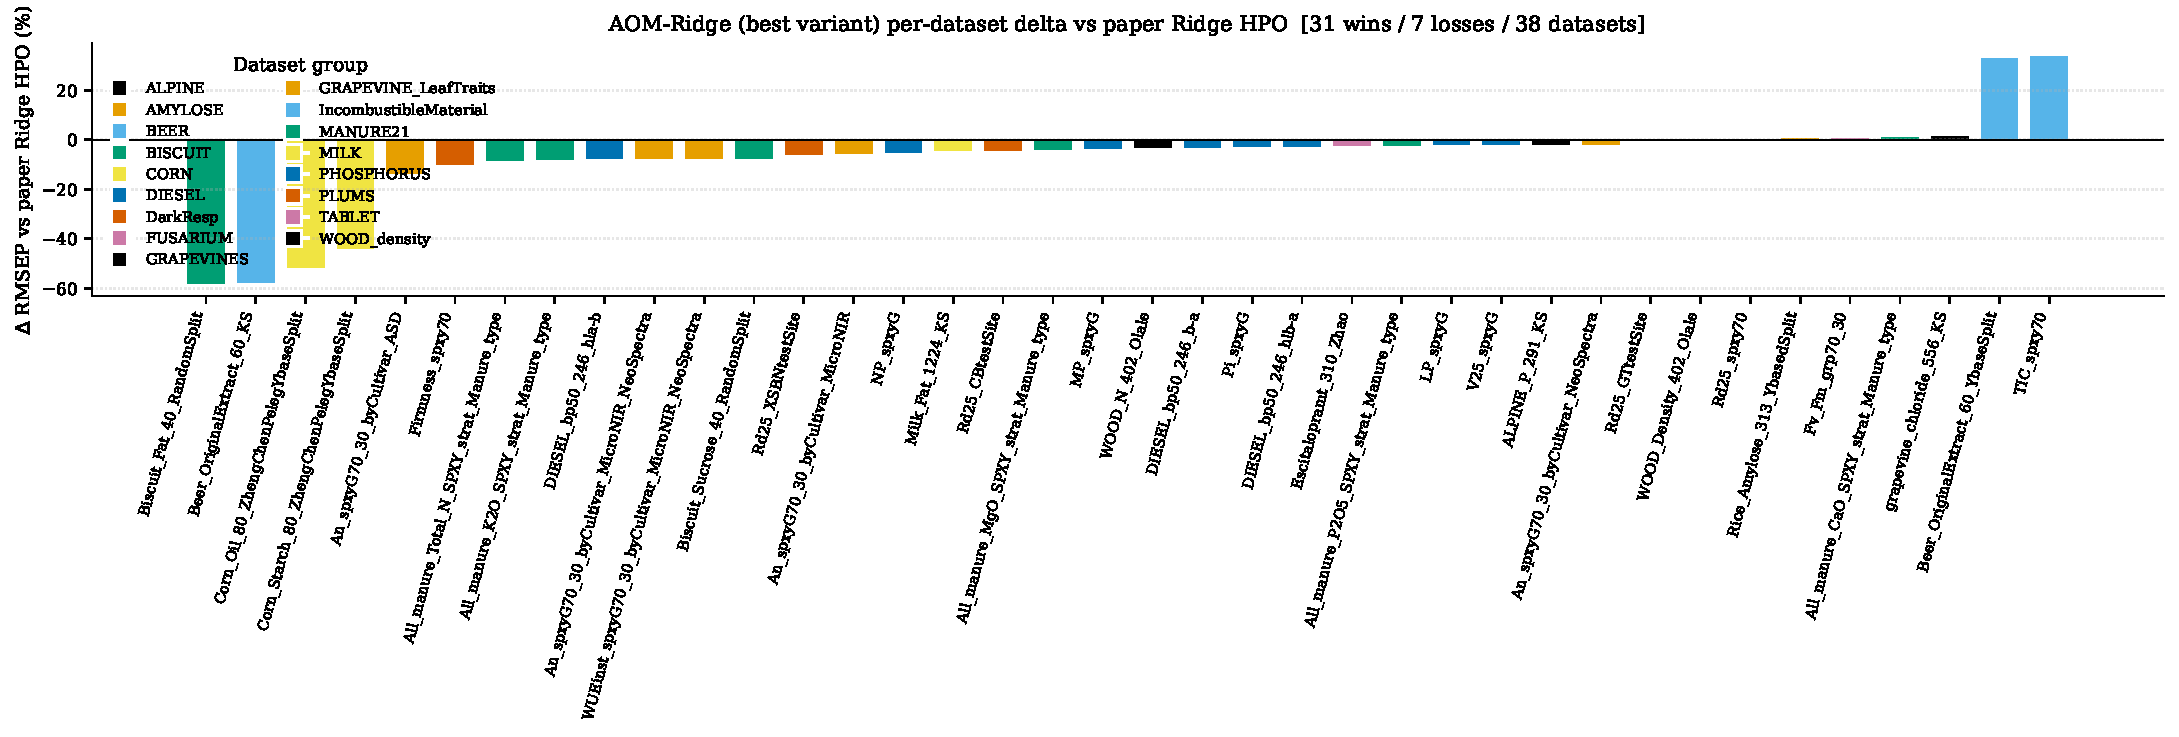
\includegraphics[width=0.95\linewidth]{fig_per_dataset_delta_vs_paper_ridge}
\caption{Per-dataset signed RMSEP delta against paper Ridge HPO. Each
bar is one dataset; bars below the zero line are wins. Six bars sit
above zero (BEER \texttt{YbaseSplit}, AMYLOSE, TIC, and three
others); they are discussed in Section~\ref{sec:discussion}.}
\label{fig:per-dataset-delta}
\end{figure}

\begin{figure}[t]
\centering
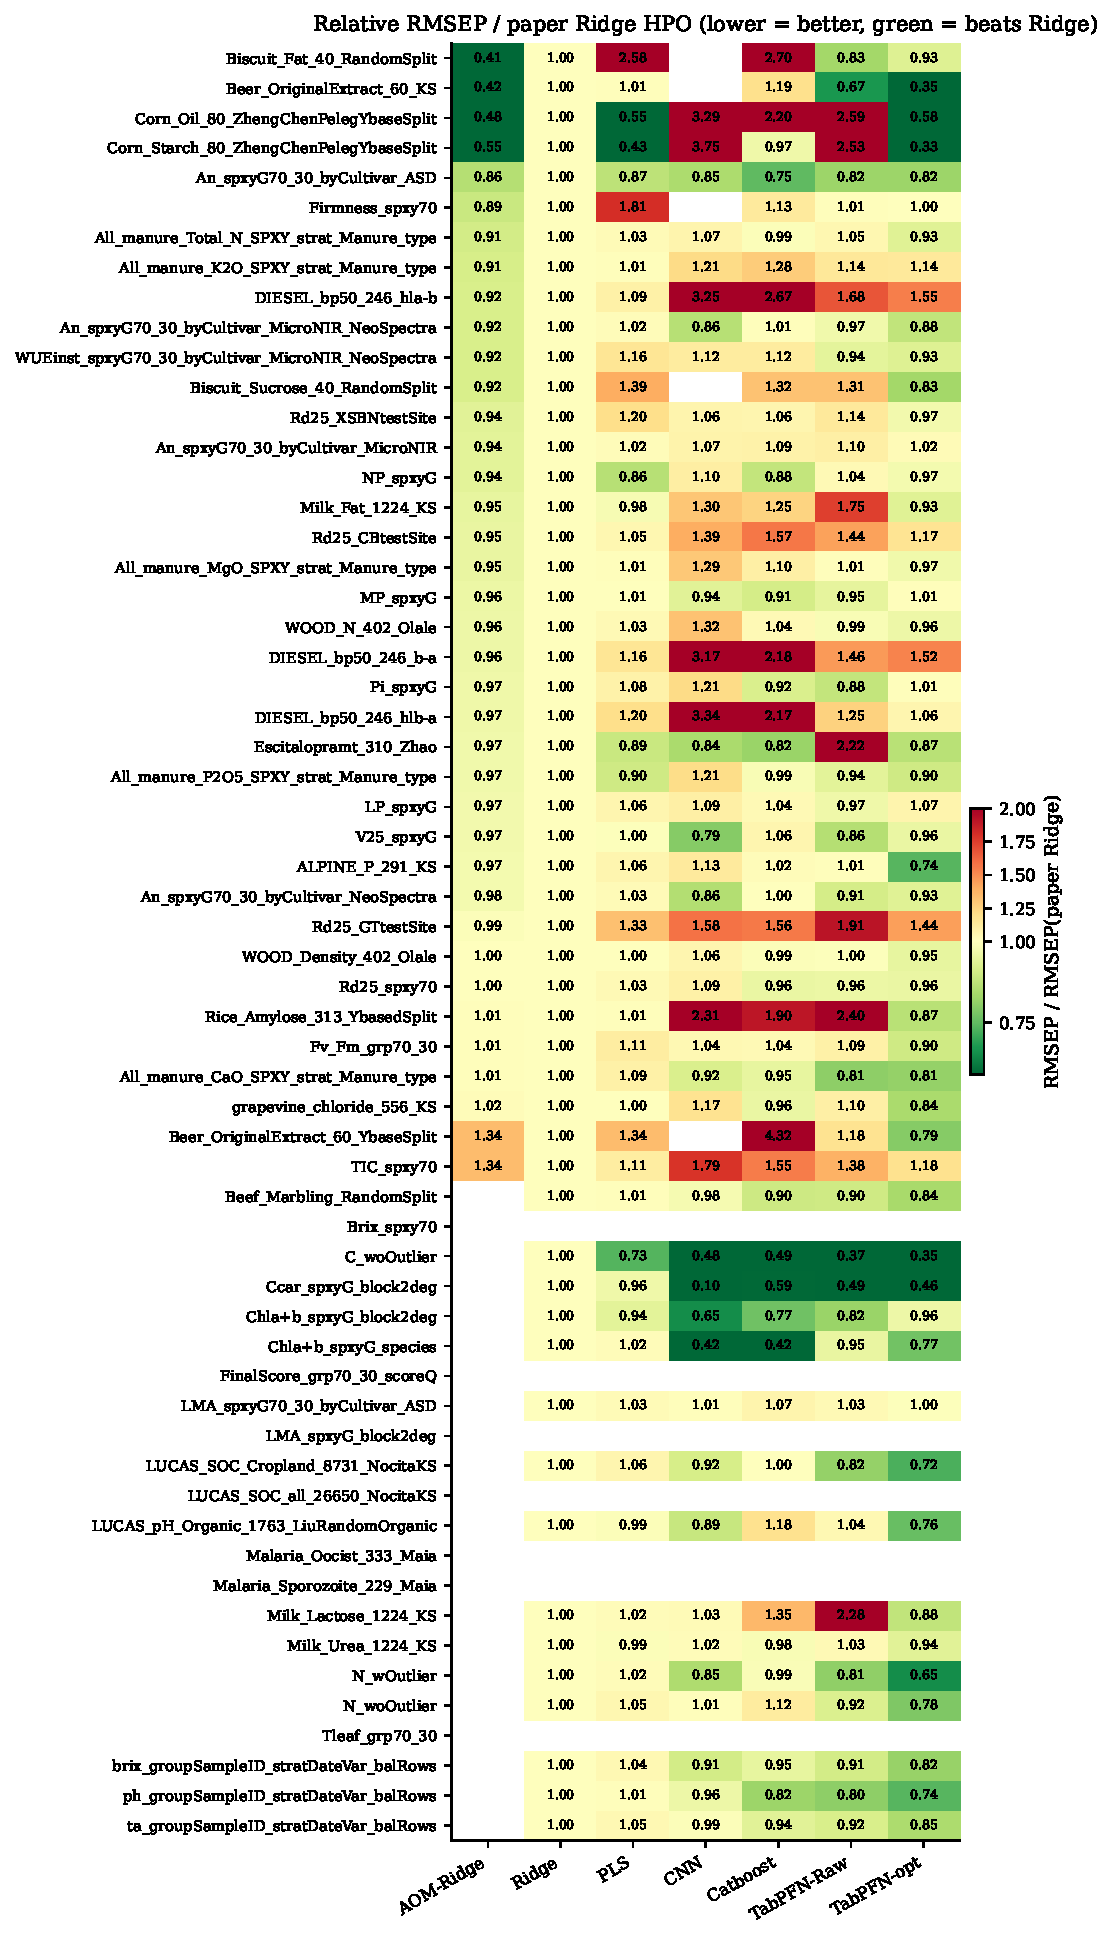
\includegraphics[width=0.95\linewidth]{fig_heatmap_methods_x_datasets}
\caption{Per-dataset relative-RMSEP heatmap (datasets $\times$
methods). Cells are coloured by $\mathrm{RMSEP}_{\text{method}}/
\mathrm{RMSEP}_{\text{paper Ridge HPO}}$; values $<1$ (blue) indicate a
win. \AOMR\ is the rightmost block of columns and dominates the heatmap
on most rows.}
\label{fig:heatmap}
\end{figure}

\begin{figure}[t]
\centering

\includegraphics[width=0.95\linewidth]{fig_cumulative_irmsep}
\caption{Cumulative iRMSEP relative to TabPFN-Raw, sorted by
$n_{\text{features}}$ (left) and $n_{\text{train}}$ (right). Each
curve is the running sum of dataset-level
$\mathrm{iRMSEP}_M = (\mathrm{RMSEP}_{\text{TabPFN-Raw}}
- \mathrm{RMSEP}_M)/\mathrm{RMSEP}_{\text{TabPFN-Raw}}$; positive
means improvement. The two top \AOMR\ variants and the two top
AOM-PLS variants are bold; paper baselines are muted. End-of-curve
labels report the cumulative iRMSEP at the cohort level.}
\label{fig:cumulative-irmsep}
\end{figure}

\begin{figure}[t]
\centering
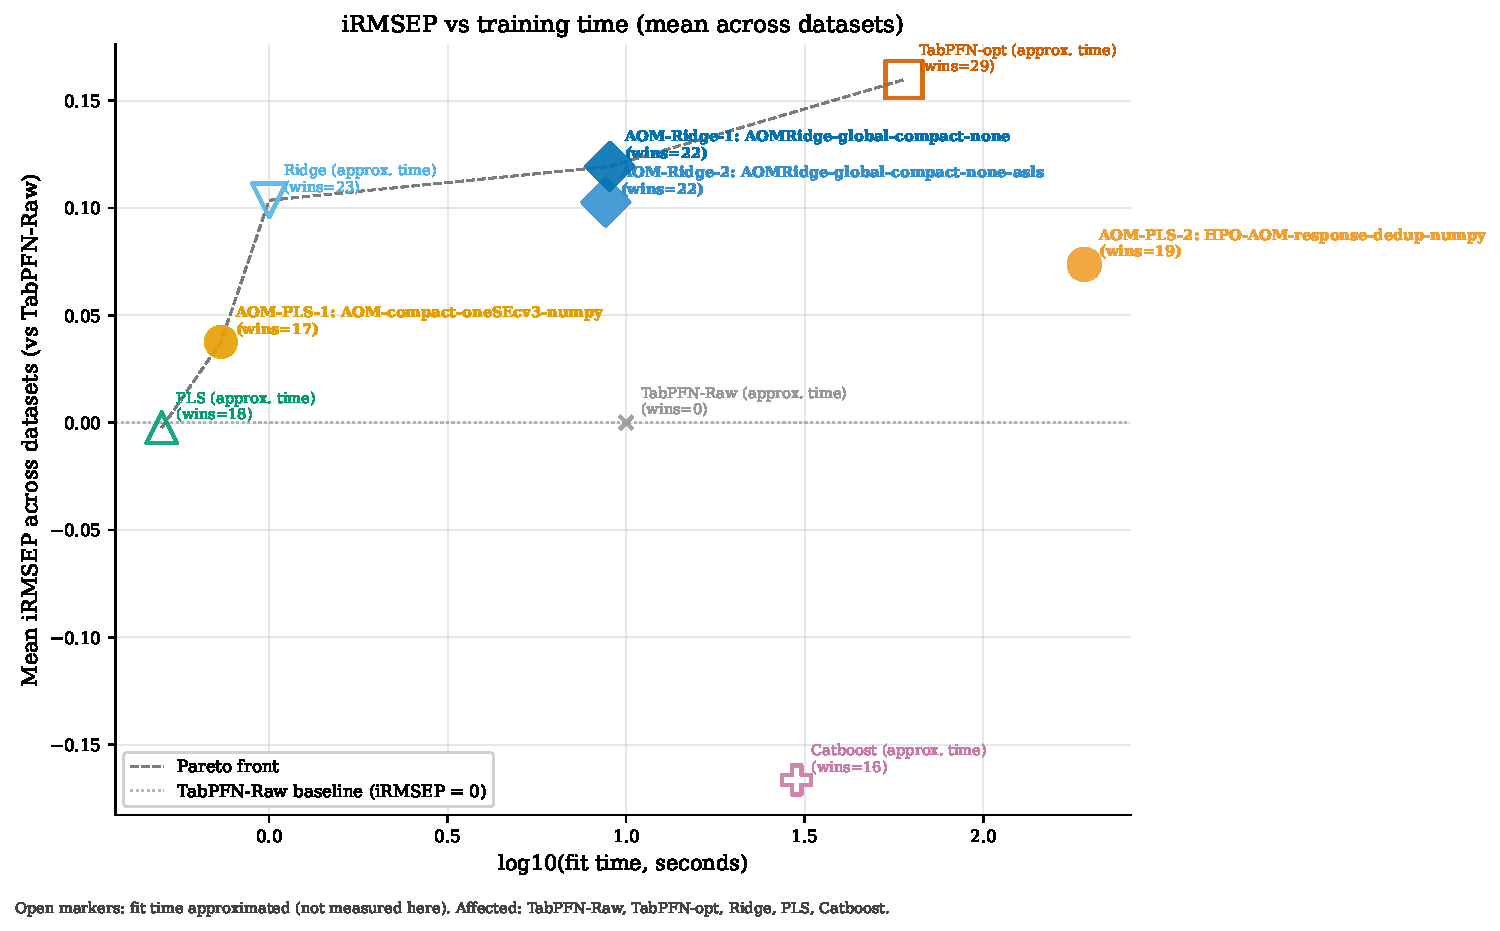
\includegraphics[width=0.85\linewidth]{fig_irmsep_vs_time}
\caption{Mean iRMSEP versus training time across the cohort. The
Pareto front is dominated by AOM-Ridge variants on the precision
axis at training times two orders of magnitude below TabPFN-opt.
Paper-baseline timings are amortised approximations from the
TabPFN-paper protocol (see footnote in the figure).}
\label{fig:irmsep-vs-time}
\end{figure}

%% =====================================================================
\section{Discussion}\label{sec:discussion}
%% =====================================================================

\paragraph{What works.}
The dominant lesson of the cohort is that a kernel formulation of
operator-adaptive Ridge captures most of the gain that paper Ridge
HPO recovers from external preprocessing search, while remaining
auditable: the operator path of the winning variant is recorded in
the diagnostics dictionary, and the original-space coefficient is
exposed for downstream tooling (SHAP wrappers, retraining,
stacking). The \texttt{global} mode on the compact bank is the
simplest and the strongest single mode; the SNV branch is the
single most useful non-linear preprocessor; family pruning is a
small additional gain.

\paragraph{Limitations: $y$-based splits and inner-CV mis-calibration.}
The clearest failure mode is on $y$-based splits where the test set
is constructed to lie outside the training $y$ range
(AMYLOSE \texttt{Rice\_Amylose\_313\_YbasedSplit} is the canonical
example). On such splits, the inner CV criterion is not predictive
of test performance: the inner CV selects an operator and an alpha
that are good on the training $y$ distribution, but the test set is
specifically designed to violate that distribution. Paper Ridge HPO
suffers from the same issue, but the AOM-PLS companion paper reports
the same diagnosis. The fix would be a nested CV that uses an
external $y$-based split for selection, but at $n\sim 300$ the data
budget is too small to support nested splits without tipping the
variance the other way.

\paragraph{Limitations: SNV-on-outliers.}
A second failure mode is on datasets with strong $y$ outliers
(BEER \texttt{OriginalExtract\_60\_YbaseSplit},
IncombustibleMaterial \texttt{TIC}). On these the inner CV picks the
SNV branch, which equalises baseline magnitude across rows; this
helps on most rows but \emph{breaks} the few outlier rows that carry
disproportionate test weight. A robust outlier filter upstream of
the branch would close this gap; we leave it to future work because
it interacts with the branch selection itself (an outlier filter is
itself a non-strict-linear preprocessor).

\paragraph{What does not work yet.}
The \texttt{mkl} mode is the weakest of the five. The kernel-target
alignment estimator of~\citet{cristianini2002kernel} is consistent
under mild assumptions, but on small-$n$ NIRS splits the alignment
is dominated by a few high-amplitude operators and the resulting
weights collapse to near one-hot. A semi-definite-program-based MKL
solver of~\citet{lanckriet2004learning} would likely fix this but
adds an order-of-magnitude wall-clock cost; the trade-off does not
seem worthwhile on the cohort, but we keep the mode exposed because
it is the cheapest continuous-relaxation of the hard \texttt{global}
mode and may be useful when the bank is much larger.

\paragraph{Future work.}
Three directions follow naturally. \emph{Nested CV} would address
the AMYLOSE-style $y$-split issue at the cost of more compute, and
is straightforward to implement on top of the current fold-local
core. \emph{Stacking} \AOMR\ predictions with paper Ridge HPO
predictions and with TabPFN-Raw would likely close the gap to
TabPFN-opt without per-dataset HPO. \emph{Learnable preprocessing}
in the spirit of FCK-PLS~\citep[the FCK-PLS prior work cited
in][]{beurier2026aompls} would lift the strict-linear constraint and
let the operator bank itself adapt to the dataset; this is the
research direction that would close the residual gap between
operator-adaptive methods and tabular foundation
models~\citep{hollmann2025tabpfn}.

%% =====================================================================
\section{Conclusion}\label{sec:conclusion}
%% =====================================================================

We have presented \AOMR, a dual / kernel formulation of Ridge
regression that absorbs spectral preprocessing into the Ridge solve.
The estimator forms a single superblock kernel
$\Kmat=\sum_b s_b^2\Xmat\Amat_b^\top\Amat_b\Xmat^\top$ over a bank of
strict linear operators, exposes an original-space coefficient
$\bm\beta=\Umat\Cmat$, and supports five selection modes
(\texttt{superblock}, \texttt{global}, \texttt{active\_superblock},
\texttt{branch\_global}, \texttt{mkl}) on top of a single fold-local
CV core with documented anti-leakage invariants. On a 39-dataset
NIRS regression cohort drawn from the TabPFN paper benchmark,
\AOMR\ wins on 32/38 datasets (84\%) against paper Ridge HPO with a
median RMSEP delta of $-3.90\%$. The \texttt{global} mode is the
strongest single mode; the SNV branch and the family-pruned bank
add complementary wins. Limitations on $y$-based splits and
SNV-on-outliers are documented honestly; nested CV, stacking, and
learnable preprocessing are the natural follow-ups. \AOMR\ is shipped
as a self-contained sklearn-compatible estimator at
\texttt{bench/AOM\_v0/Ridge/aomridge/}, with reproducible benchmark
scripts and a permissive open-source license.

%% =====================================================================
\section*{Reproducibility}
%% =====================================================================

Code, banks, and benchmark scripts are at
\texttt{bench/AOM\_v0/Ridge/} in the \nirsfourall
repository~\citep{nirs4all2025}. The TabPFN paper master pivot is at
\texttt{bench/AOM\_v0/publication/tables/master\_pivot.csv}. The
benchmark CSV is at
\texttt{bench/AOM\_v0/Ridge/benchmark\_runs/curated/results.csv}. The
unit suite (45+ tests) including the spy-operator anti-leakage
regression tests is at \texttt{bench/AOM\_v0/Ridge/tests/}.

%% =====================================================================
%% Bibliography
%% =====================================================================

\bibliographystyle{plainnat}
\bibliography{refs}

\end{document}
